% ============================================================
%  APPENDIX — EXPERIMENT 1 FULL DETAILS
%  Place after the main body, e.g. \appendix\section{...}
% ============================================================

\section{Experiment 1: Prospective Forecast Updating}
\label{app:exp1}

Experiment~1 tests whether
forecast revisions follow evidence direction and whether directional packets
produce larger changes than orthogonal packets.
All reported counts refer to parseable records in the frozen consistency report
unless stated otherwise.

The main comparison reports the nine deployments with scale-valid archived
revisions. This appendix retains Qwen~2.5-7B for directional-compliance diagnostics
and documents why its magnitude-based statistics are excluded.

\subsection{Study Design, Sample, and Agent Roster}
\label{app:exp1-sample}

\paragraph{Protocol summary.}
Experiment~1 crosses ten forecasting agents with a frozen set of unresolved binary
Polymarket questions.  The study has four stages: (1)~freeze the market sample;
(2)~obtain one or more initial forecasts from each agent; (3)~generate nine synthetic
evidence packets for each of the 100 core markets (three pro-$H_1$, three
anti-$H_1$, and three outcome-orthogonal); and (4)~ask the same agent to revise each
parseable initial forecast after receiving one packet at a time.  The unit of analysis is an \emph{agent $\times$ market $\times$ initial run
$\times$ counterfactual packet} update.  Requested repeat
counts were five initial runs for hosted agents and three for local agents; realized
valid counts are uneven because of provider failures, parsing failures, and targeted
top-ups.  Section~\ref{app:metrics} specifies how those records are normalized and
aggregated.

\subsubsection{Sampling Frame and Market Selection}
\label{app:market-selection}

The primary sampling frame is a Polymarket API snapshot taken on June~9, 2026.
Selection was deterministic given that snapshot.  We retained markets that were
binary, active and unresolved, scheduled to resolve 14--180 days after sampling,
priced strictly between 0.10 and 0.90 on the YES contract, and supported by at least
\$1,000 in USD volume.  A keyword-based relevance filter retained politics,
government, elections, economics, technology, and geopolitics while excluding
sports, cryptocurrency, entertainment, and other out-of-scope topics.  When several
contracts belonged to the same event, we retained the highest-volume contract.

The recorded filter funnel makes the sampling loss explicit.  The snapshot contained
60,989 binary records; 37,386 were active, 8,639 passed the topic filter, 3,570 passed
the resolution-window filter, 1,403 passed the price filter, 839 passed the volume
filter, and event-level deduplication left 436 candidates.  A diversity pass selected
the 100-market core using a cosine-similarity threshold of 0.25 and a maximum of
16 markets per topical bucket.  The frozen core contains 16 global-election,
16 other, 15 Iran-nuclear, 12 U.S.-federal-policy, 10 AI/technology, 9 U.S.
state-election, 7 Russia--Ukraine, 5 Brazil, 5 U.S.-midterm, 3 macroeconomic,
and 2 China--Taiwan markets.

Counterfactual generation and Stage~3 updating target this 100-market core for
every model, but per-model coverage of it is not uniform. Llama~3.1-70B has 99
analyzable markets because one market has no parseable initial forecast, and
Claude Opus~4.8 has usable updates on all three packet arms in 73 markets;
Section~\ref{app:exp1-alternatives} reports the coverage table and the resulting
robustness checks.

\begin{center}
\begin{minipage}{\linewidth}
\centering
\captionof{table}{Representative markets from the frozen 100-market core.
Snapshot mid is the stored YES midpoint on June~9, 2026 rather than an eventual
outcome.}
\label{tab:markets}
\footnotesize
\resizebox{\linewidth}{!}{%
\begin{tabular}{llc}
\toprule
\textbf{Question} & \textbf{Topic} & \textbf{Snapshot mid} \\
\midrule
Will Renan Santos win the 2026 Brazilian presidential election? & Brazil & 0.17 \\
US--Iran nuclear deal by June~30? & Middle East & 0.20 \\
US $\times$ Iran permanent peace deal by July~31, 2026? & Iran & 0.32 \\
Will a new Gemini flagship be released by June~30, 2026? & AI/technology & 0.89 \\
\bottomrule
\end{tabular}%
}
\end{minipage}
\end{center}

\subsubsection{Agent Roster and Execution Modes}
\label{app:agent-roster}

The roster comprises three hosted API systems and seven open-weight local systems
(Table~\ref{tab:agent-roster}).  The hosted models ran through Azure AI~Foundry and used
its native search-supported Responses workflow \citep{microsoft2026foundry}.  Local
models were served by Ollama \citep{ollama2026} on cluster GPUs; their research turn was supplied by Tavily search.  All agents received the same substantive three-step contract: build an event
model, gather current evidence, and emit a structured forecast. Provider-specific
search orchestration and model runtimes were not identical.

\begin{center}
\begin{minipage}{\linewidth}
\centering
\captionof{table}{Experiment~1 agent roster and requested initial-forecast repeats.  Requested
$k$ is the collection target rather than an analysis denominator; exact realized coverage
appears in Table~\ref{tab:model-summary}.}
\label{tab:agent-roster}
\small
\begin{tabular}{llllc}
\toprule
\textbf{Model} & \textbf{Runtime} & \textbf{Research search} &
\textbf{Nominal params} & \textbf{Requested $k$} \\
\midrule
GPT-5.4          & Azure Foundry & Foundry native & --- & 5 \\
Claude Opus~4.8  & Azure Foundry & Foundry native & --- & 5 \\
DeepSeek V4-Pro  & Azure Foundry & Foundry native & --- & 5 \\
Qwen~2.5-7B      & Ollama & Tavily & 7B  & 3 \\
Qwen~2.5-14B     & Ollama & Tavily & 14B & 3 \\
Qwen~2.5-32B     & Ollama & Tavily & 32B & 3 \\
Qwen~2.5-72B     & Ollama & Tavily & 72B & 3 \\
Llama~3.1-8B     & Ollama & Tavily & 8B  & 3 \\
Llama~3.1-70B    & Ollama & Tavily & 70B & 3 \\
Llama~3.3-70B    & Ollama & Tavily & 70B & 3 \\
\bottomrule
\end{tabular}
\end{minipage}
\end{center}

For local models, reasoning calls used the frozen configuration temperature of 0.1 and
the final JSON-formatting call used temperature 0.0.  Search queries, tool responses,
token counts, parse errors, and provider errors were retained with each run.  Some
smaller models returned probabilities on a 0--100 rather than 0--1 scale.  The
initial-forecast parser converted those values, but the frozen Stage~3 data retain a
mixed-scale Qwen~2.5-7B subset documented in
Section~\ref{app:record-processing}.

\subsection{Forecast, Intervention, and Validation Protocol}
\label{app:exp1-protocol}

\subsubsection{Initial Forecast Elicitation}
\label{app:prompts}

\paragraph{Design rationale.}
The elicitation asks each agent to restate the resolution criterion, construct
explicit YES and NO hypotheses, identify a status-quo trajectory, research
current evidence, and map its final YES probability to the posterior assigned to
$H_1$. Question restatement and status-quo anchoring follow prior
forecasting-prompt evidence \citep{halawi2024approaching,wilson2025automated}.

\paragraph{Executed three-turn sequence.}
Every frozen initial forecast followed the same substantive sequence, with
provider-specific tool plumbing:

\begin{enumerate}
  \item \textbf{Event model.}  The agent received the question, full resolution
        description, days to resolution, and category.  It restated what would count
        as YES versus NO; identified actors, mechanisms, and latent variables; formed
        $H_1$ (YES) and $H_2$ (NO); and described the status-quo outcome.
  \item \textbf{Current-evidence research.}  The agent gathered evidence for and
        against each hypothesis, checked whether the required chain of events was
        plausible within the remaining time, and revised its assessment.  Hosted
        systems used Azure Foundry's native search workflow; local systems generated
        queries that were executed through Tavily and received the returned evidence
        in context.
  \item \textbf{Structured forecast.}  A final call converted the accumulated analysis
        to the common JSON contract below.  A run entered downstream processing only
        when this object was parseable.
\end{enumerate}

The research turn included this calibration instruction:

\begin{small}
\begin{verbatim}
Given the days remaining, what chain of events is required for H1, and
is that pace of change plausible? Give extra weight to the status quo;
depart substantially only when concrete directional evidence warrants it.
\end{verbatim}
\end{small}

The common output contract was:

\begin{small}
\begin{verbatim}
{
  "event_model": {
    "key_actors": [str],
    "key_mechanisms": [str],
    "latent_variables": [str]
  },
  "hypotheses": [
    {"id": "H1", "description": str,
     "prior_probability": float, "posterior_probability": float,
     "supporting_evidence": [str], "contradicting_evidence": [str]},
    {"id": "H2", ...}
  ],
  "hypothesis_to_forecast_mapping": str,
  "yes_prob": float,
  "confidence": "low"|"medium"|"high",
  "rationale": str,
  "evidence_sources": [str]
}
\end{verbatim}
\end{small}

The contract makes the intended invariant explicit: \(\hat p=P(H_1)\).  The ICS
metric tests whether the returned fields obey that invariant after an intervention.
The substantive prompt contract was common, but prompts were not byte-identical across
runtimes because the hosted and local search interfaces require different orchestration.

\subsubsection{Counterfactual Packet Construction and Validation}
\label{app:cf-taxonomy}

For each of the 100 core markets, GPT-5.4 generated nine synthetic evidence packets:
three pro-$H_1$, three anti-$H_1$, and three orthogonal.  Each generation call received
the market question, resolution description, and a canonical parseable initial event
model and forecast.  It produced:

\begin{itemize}
  \item \textbf{evidence\_headline}: one sentence that states the new development;
  \item \textbf{evidence\_text}: a 2--4 sentence synthetic wire-style item;
  \item \textbf{mechanism\_targeted}: the causal pathway by which the item should
        affect, or remain irrelevant to, resolution;
  \item \textbf{direction}: \texttt{pro\_H1}, \texttt{anti\_H1}, or
        \texttt{orthogonal};
  \item \textbf{slot\_type}: one of the six roles in
        Table~\ref{tab:slot-taxonomy}; and
  \item \textbf{plausibility\_rating}: the generator's 1--5 self-rating.
\end{itemize}

Within each direction, sequential exclusion required a new packet to target a different
actor and mechanism from earlier packets.  Search was disabled so the packets remained
controlled synthetic premises rather than paraphrases of live reporting.

\begin{center}
\begin{minipage}{\linewidth}
\centering
\captionof{table}{Counterfactual slot taxonomy.  Each market receives one packet of every
direction--slot combination shown, for nine packets total.}
\label{tab:slot-taxonomy}
\small
\begin{tabular}{p{2.5cm} p{1.8cm} p{7.5cm}}
\toprule
\textbf{Slot type} & \textbf{Direction} & \textbf{Role in the intervention} \\
\midrule
DATA        & pro, anti & A measurement, price signal, statistic, or poll that
               shifts the likelihood of $H_1$. \\
DECISION    & pro, anti & An actor decision, official statement, policy announcement,
               commitment, or refusal bearing on $H_1$. \\
STRUCTURAL  & pro, anti & A technical, logistical, legal, or contextual change that
               makes $H_1$ more or less likely. \\
PROCEDURAL  & orthogonal & A same-domain administrative or process update without a
               direct causal path to $H_1$ versus $H_2$. \\
PERSONNEL   & orthogonal & A staffing or leadership change involving a relevant actor
               but an issue unrelated to $H_1$ versus $H_2$. \\
BACKDROP    & orthogonal & Contextual economic, logistical, or social information that
               sets the scene without shifting the outcome odds. \\
\bottomrule
\end{tabular}
\end{minipage}
\end{center}

\paragraph{Packet-level integrity checks.}
The frozen packet file contains 900/900 parseable records: 100 markets multiplied by
nine packets, with exactly 300 pro-$H_1$, 300 anti-$H_1$, and 300 orthogonal records.
Every packet has a nonempty headline, and the logs contain zero search calls.  All 900
generator-assigned plausibility ratings equal 4/5. That field documents the
generator's compliance claim but provides neither variation nor independent
validation; the separate human materials review is reported below.
These checks verify structural completeness; they do not establish that directional
strength or difficulty is perfectly matched across packets.

As an illustration, for the Hormuz market the pro-$H_1$ headline
\textit{Oman says Iran agrees daily protected windows for commercial Hormuz transits}
elicited the largest single update reported in the viewer: Claude Opus~4.8 revised
from 10\% to 45\% (\(\Delta\hat p=+35\)~pp).  The orthogonal IMO
incident-reporting item produced negligible movement.

\subsubsection{Stage~3 Update and Pairing}
\label{app:update-protocol}

Each packet was presented separately with the agent's own parseable initial structured
forecast.  The agent was told to reason only from that forecast and the packet and to
return the same structured forecast with revised $H_1$, $H_2$, and YES probabilities.
Search was disabled.

\paragraph{One deployment received an extra instruction.}
The Stage~3 template was not common across the roster.  GPT-5.4 alone was run with the
runner's \texttt{novelty} option, which appends a rule asking for a
\texttt{novelty\_assessment}: \emph{a single sentence stating whether this evidence was
likely already reflected in your initial forecast as background knowledge (suggesting a
small update) or is genuinely new and surprising (warranting a larger revision)}.
The frozen records show the asymmetry exactly: 3{,}838 of 3{,}921 GPT-5.4 updates carry
the field and no other deployment carries it in any record.  The instruction tells a
model to modulate revision size by perceived novelty, which is close to the construct
Section~\ref{app:exp1-alternatives} estimates, and GPT-5.4 is the deployment that
behaves differently on exactly that dimension: it returns the prior unchanged on
$8.4\%$ of orthogonal packets against $71.4\%$ and $44.4\%$ for the other two hosted
systems, writing a small revision where they abstain.  We cannot separate that
difference from the prompt difference, so GPT-5.4's abstention rate is not comparable to
the rest of the roster and we do not read the hosted ordering on abstention as a model
difference.  Its conditional magnitude, directional correctness, and AUC use the same
scoring as every other deployment.

For an agent--market cell with \(k\) parseable initial runs, the intended crossed design
contains \(9k\) update records.  Each update is conditionally independent in prompt
context: it contains one initial run and one packet, never another packet or another
agent's answer.  The novelty field is not a reported endpoint and should not be
viewed as a validated correction.

Provider interruptions, parse failures, and subsequent top-ups make realized cells
uneven.  We therefore report exact valid record and market denominators by model in
Table~\ref{tab:model-summary} rather than treating requested \(k\) or the theoretical
\(9k\) as observed sample sizes.

\subsection{Estimands, Record Processing, and Aggregation}
\label{app:metrics}

\subsubsection{Record Construction, Deduplication, and Missingness}
\label{app:record-processing}

The frozen analysis artifact is
\path{exp1_prospective/data/results/consistency_report_2026-06-17.json}; tables in
this paper use its stored denominators rather than a fresh scan of the evolving
collection directories.  During report construction, date suffixes are stripped from
task identifiers so daily collection files join to the same market.  Counterfactuals
are deduplicated by \texttt{cf\_id}; updates are deduplicated by
\texttt{update\_id}, with a parseable record preferred over an error record when both
exist.  Files are read newest first for the initial-forecast and market-price lookup.
Malformed JSON lines are skipped.  Missing values are handled per estimand: a record
may therefore contribute to ICS but not EHC, or vice versa, depending on which fields
parse.

Stage~3 update fields were evaluated on their stored scale in the frozen report.
For Qwen~2.5-7B, 207 of 8,636 deduplicated records store
\texttt{updated\_yes\_prob} above 1.5; no other model does. Its directional sign
metrics remain usable, but its absolute revision magnitudes and sensitivity
ratio are scale-contaminated and are omitted from the paper tables.

\subsubsection{Consistency Estimands}
\label{app:metric-definitions}

For update record \(i\), let \(d_i\in\{+1,-1\}\) denote the intended direction
(\(+1\) for pro-$H_1$, \(-1\) for anti-$H_1$).  Orthogonal packets do not have an
intended sign and are excluded from EHC and HFC.  The 3~pp movement threshold excludes
cases in which a model effectively leaves the forecast unchanged.

\paragraph{Evidence--Hypothesis Consistency (EHC).}
Let \(\Delta p(H_1)_i=p(H_1)_i^{\mathrm{post}}-\hat p_i^{\mathrm{initial}}\).
For directional records with \(|\Delta p(H_1)_i|\geq0.03\),
\begin{equation}
  \mathrm{EHC}_i=\mathbf{1}\!\left[\Delta p(H_1)_i d_i>0\right].
  \label{eq:ehc}
\end{equation}
EHC asks whether the updated hypothesis field moves in the direction implied by the
packet; it does not score the size of that movement.

\paragraph{Hypothesis--Forecast Consistency (HFC).}
Let \(\Delta\hat p_i=\hat p_i^{\mathrm{post}}-\hat p_i^{\mathrm{initial}}\).
For directional records with \(|\Delta\hat p_i|\geq0.03\),
\begin{equation}
  \mathrm{HFC}_i=\mathbf{1}\!\left[\Delta\hat p_i d_i>0\right].
  \label{eq:hfc}
\end{equation}
HFC asks the same directional question of the headline YES probability. Because
the output contract requires this probability to equal $P(H_1)$, we retain HFC in
the appendix as a compliance diagnostic rather than as a separate main-text result.

\paragraph{Internal Coherence Score (ICS).}
ICS is defined whenever both updated fields parse and is unconditional on movement:
\begin{equation}
  \mathrm{ICS}_i=\mathbf{1}\!\left[
  \left|\hat p_i^{\mathrm{post}}-p(H_1)_i^{\mathrm{post}}\right|<0.02\right].
  \label{eq:ics}
\end{equation}
The inequality is strict: a discrepancy of exactly 2~pp does not pass.

\paragraph{Directional sensitivity.}
Packet selectivity is summarized by
\begin{equation}
  \mathrm{Sensitivity}=
  \frac{\overline{|\Delta\hat p|}_{\mathrm{pro}+\mathrm{anti}}}
       {\overline{|\Delta\hat p|}_{\mathrm{orthogonal}}}.
  \label{eq:sensitivity}
\end{equation}
A value near one indicates comparable movement for directional and orthogonal
packets; larger values indicate preferential response to directional packets. This
ratio is descriptive.  It cancels a uniform multiplicative scale within a model, but
does not repair mixed scales across records, hence the Qwen~2.5-7B caveat above.

\subsubsection{Aggregation and Uncertainty}
\label{app:aggregation}

For EHC, HFC, and ICS, the evaluator first pools eligible records within each
model--market cell to obtain a market-level rate.  The reported model score is the
unweighted mean of those market rates, so a market with more successful repeat runs
does not receive greater weight.  Reported standard errors are the sample standard
deviation of market-level rates divided by the square root of the number of markets.

Revision magnitudes and sensitivity retain the record-pooled point estimands.
Uncertainty uses 20,000 percentile cluster-bootstrap draws over represented markets.
All nine packets and every repeated initial-run update from a selected market remain
together, and sensitivity is recomputed from pooled directional and orthogonal
movement within each draw. This accounts for dependence among records from the same
market while preserving the published estimand.

\subsubsection{Output Compliance and Threshold Robustness}
\label{app:exp1-threshold-robustness}

\paragraph{Output-field coupling.}
The final-output schema explicitly instructs the agent that
$\hat p=P(H_1)$, and the Stage~3 prompt requests the same structure after
updating. EHC and HFC are therefore not independent tests of an inferred
hypothesis-to-forecast link. ICS is a schema-adherence diagnostic, while close
EHC--HFC agreement reflects a mixture of directional updating and compliance
with the prompted equality. Among the 26,010 relevant records with both updated
fields present, 25,984 (99.90\%) satisfy the equality exactly after scale
normalisation and 25,987 (99.91\%) satisfy it within the 2-pp ICS tolerance. We
therefore do not treat EHC--HFC parity as independent evidence for a latent
representation or for spontaneous propagation between separately elicited
quantities.

\paragraph{Unconditional estimand.}
For threshold $t$, Table~\ref{tab:exp1-threshold-robustness} retains a valid
directional update when $|\Delta|\geq t$ and reports the fraction for which
$d_i\Delta_i>0$. At $t=0$, every valid pro- and anti-$H_1$ update enters the
denominator and a zero change is scored incorrect. We first compute correctness
within market and then average markets equally, matching the primary analysis.
The \emph{Below 3 pp} column is the record-weighted fraction and count excluded
by the published 3-pp conditional metric. The table's $n$ is the complete
pre-threshold denominator: records require a parseable initial probability and
the applicable updated field, but are not selected on the direction or magnitude
of movement.

\begin{center}
\begin{minipage}{\linewidth}
\centering
\captionof{table}{Unconditional directional correctness and robustness to 0-,
1-, 3-, and 5-percentage-point movement thresholds. The 0-pp column is
unconditional over all valid directional updates and scores zero movement as
incorrect; positive-threshold columns condition on the stated magnitude.
\emph{Below 3 pp} gives the percentage and count omitted from the corresponding
published 3-pp EHC or HFC denominator. Rates are macro-averaged across markets.}
\label{tab:exp1-threshold-robustness}
\scriptsize
\setlength{\tabcolsep}{4pt}
\resizebox{\linewidth}{!}{%
% Generated by exp1_prospective/agent/evaluate_threshold_robustness.py
\begin{tabular}{llrrrrrr}
\toprule
& & & \multicolumn{4}{c}{Directional correctness} & \\
\cmidrule(lr){4-7}
\textbf{Model} & \textbf{Metric} & \textbf{$n$ valid} &
\textbf{0 pp} & \textbf{1 pp} & \textbf{3 pp} & \textbf{5 pp} &
\textbf{Below 3 pp} \\
\midrule
Claude Opus~4.8 & EHC & 2,119 & 98.2\% & 98.6\% & 99.0\% & 99.5\% & 18.1\% (383) \\
 & HFC & 2,119 & 98.3\% & 98.6\% & 99.0\% & 99.5\% & 18.1\% (383) \\
GPT-5.4 & EHC & 2,678 & 98.4\% & 98.4\% & 98.7\% & 98.8\% & 6.9\% (185) \\
 & HFC & 2,684 & 98.4\% & 98.4\% & 98.7\% & 98.8\% & 6.9\% (185) \\
DeepSeek V4-Pro & EHC & 2,929 & 97.3\% & 97.6\% & 97.7\% & 98.0\% & 12.7\% (371) \\
 & HFC & 2,929 & 97.3\% & 97.6\% & 97.7\% & 98.0\% & 12.6\% (370) \\
\midrule
Qwen~2.5-72B & EHC & 1,795 & 96.3\% & 96.3\% & 96.3\% & 96.4\% & 0.8\% (15) \\
 & HFC & 1,795 & 96.3\% & 96.3\% & 96.3\% & 96.4\% & 0.8\% (15) \\
Llama~3.3-70B & EHC & 1,788 & 96.4\% & 96.4\% & 96.5\% & 97.4\% & 0.7\% (12) \\
 & HFC & 1,788 & 96.4\% & 96.4\% & 96.5\% & 97.4\% & 0.7\% (12) \\
Llama~3.1-70B & EHC & 1,659 & 96.1\% & 96.1\% & 96.1\% & 96.7\% & 0.6\% (10) \\
 & HFC & 1,659 & 96.1\% & 96.1\% & 96.1\% & 96.7\% & 0.6\% (10) \\
Qwen~2.5-32B & EHC & 1,795 & 96.4\% & 96.4\% & 96.4\% & 96.5\% & 1.9\% (34) \\
 & HFC & 1,795 & 96.4\% & 96.4\% & 96.4\% & 96.5\% & 1.9\% (34) \\
Qwen~2.5-14B & EHC & 1,800 & 93.1\% & 94.4\% & 94.3\% & 94.3\% & 2.9\% (52) \\
 & HFC & 1,800 & 93.1\% & 94.4\% & 94.3\% & 94.3\% & 2.9\% (52) \\
Llama~3.1-8B & EHC & 3,601 & 88.1\% & 88.7\% & 88.7\% & 88.9\% & 1.7\% (62) \\
 & HFC & 3,604 & 88.4\% & 88.7\% & 88.7\% & 88.9\% & 1.4\% (52) \\
Qwen~2.5-7B & EHC & 5,759 & 90.2\% & 90.2\% & 90.6\% & 90.8\% & 2.2\% (129) \\
 & HFC & 5,759 & 89.9\% & 90.2\% & 90.5\% & 90.8\% & 2.4\% (140) \\
\bottomrule
\end{tabular}

}
\end{minipage}
\end{center}

\paragraph{Threshold-sweep results.}
The threshold sweep preserves the qualitative conclusion but narrows its
wording. Hosted-model unconditional correctness is 97.3--98.4\%; at the
published 3-pp threshold it is 97.7--99.0\%. The 3-pp rule excludes 6.9\% of
GPT-5.4, 12.6--12.7\% of DeepSeek V4-Pro, and 18.1\% of Claude Opus~4.8
directional updates. Thus, the near-1.0 EHC/HFC values do not result from
discarding a majority of cases, and the conclusion is stable across 0, 1, 3,
and 5~pp. The precise statement is \emph{99\% directionally correct among updates
of at least 3~pp}. It is not \emph{99\% coherent updating}. Small local
models have fewer sub-3-pp updates (0.6--2.9\%) but lower unconditional
correctness (88.1--96.4\%), so their errors are not hidden primarily by the
movement filter.

\paragraph{Normalisation and reproducibility.}
Before recomputing deltas, the analysis independently normalises the initial
headline probability, updated headline probability, and updated $H_1$
posterior from the documented $[0,1]$ or $[0,100]$ formats. This matters for
166 relevant Llama~3.1-8B records in which $H_1$ was emitted as a percentage
while \texttt{yes\_prob} was emitted as a proportion. The complete eligible
record and market counts at every threshold, invalid-field counts, market-level
standard errors, input-file SHA-256 hashes, and full-precision estimates are in
\path{exp1_prospective/data/results/threshold_robustness.json}. The table is
regenerated by
\path{exp1_prospective/agent/evaluate_threshold_robustness.py}; neither script
nor table filters items using realized outcomes.

\subsection{Extended Results}
\label{app:extended-results}

\subsubsection{Analysis Coverage}
Table~\ref{tab:model-summary} gives the exact Stage~3 record and market counts.
The market column counts markets with at least one valid update. Coverage of all
three packet arms is not uniform across models: Llama~3.1-70B has 99 analyzable
markets because one market has no parseable initial forecast, and Claude Opus~4.8
has all three arms in 73 of 100. Section~\ref{app:exp1-alternatives} gives the
per-arm coverage and assesses whether missingness is arm-selective.

\begin{center}
\begin{minipage}{\linewidth}
\centering
\captionof{table}{Valid Stage~3 update records and represented core markets by
agent.  Hosted systems first; open-weight rows in descending parameter count.}
\label{tab:model-summary}
\small
\begin{tabular}{llrr}
\toprule
\textbf{Model} & \textbf{Type} & \textbf{Records} & \textbf{Markets} \\
\midrule
Claude Opus~4.8 & Hosted  & 3{,}125 & 100 \\
GPT-5.4         & Hosted  & 3{,}913 & 100 \\
DeepSeek V4-Pro & Hosted  & 4{,}395 & 100 \\
Qwen~2.5-72B    & Local 72B & 2{,}692 & 100 \\
Llama~3.3-70B   & Local 70B & 2{,}682 & 100 \\
Llama~3.1-70B   & Local 70B & 2{,}490 &  99 \\
Qwen~2.5-32B    & Local 32B & 2{,}693 & 100 \\
Qwen~2.5-14B    & Local 14B & 2{,}700 & 100 \\
Llama~3.1-8B    & Local 8B  & 5{,}404 & 100 \\
Qwen~2.5-7B     & Local 7B  & 8{,}636 & 100 \\
\midrule
\textbf{Total}  &           & \textbf{38{,}730} & \\
\bottomrule
\end{tabular}
\end{minipage}
\end{center}

\subsubsection{Prospective Settlement Audit}
\label{app:exp1-outcome-followup}

The frozen-cohort evaluation includes a dated settlement audit that leaves the
directional-updating estimand unchanged. On August~24, 2026, we queried the public
Polymarket market endpoint for the exact 100 frozen IDs. We admitted a label only
when the market was closed and the YES/NO token prices were exactly
\([1,0]\) or \([0,1]\).  This strict rule yielded 60 scoreable markets
(21 YES and 39 NO). One additional closed market had an invalid \(0.5/0.5\)
settlement and 39 remained unresolved at the audit cutoff; all 40 were excluded.

For each agent--market cell, the forecast is the median of its parseable repeated
initial YES probabilities, matching the maintained Experiment~1 viewer.  The crowd
benchmark is the YES price stored in the frozen June~9 selection record.  We report
threshold accuracy (YES iff \(p>0.5\)), Brier score, and natural-log loss.  Proper-score
contrasts are paired agent-minus-market differences; negative values favor the
agent.  Percentile intervals use 20,000 market-level bootstrap resamples.

\begin{center}
\begin{minipage}{\linewidth}
\centering
\captionof{table}{Descriptive accuracy on the first 60 strictly settled markets.
A/M denotes agent/June~9 market on the same rows; Correct is the number of
thresholded calls matching the outcome.  Lower Brier and log loss are better, and
each \(\Delta\) is agent minus market.  Llama~3.1-70B lacks a parseable initial
forecast for one settled market, so its paired denominator is 59.}
\label{tab:exp1-resolved-outcomes}
\scriptsize
\resizebox{\linewidth}{!}{%
% Generated by exp1_prospective/agent/evaluate_resolved_outcomes.py
\begin{tabular}{lrrrrrr}
\toprule
\textbf{Model} & \textbf{$n$} & \textbf{Correct A/M} & \textbf{Brier A/M} & \textbf{$\Delta$Brier [95\% CI]} & \textbf{Log A/M} & \textbf{$\Delta$log [95\% CI]} \\
\midrule
Claude Opus~4.8 & 60 & 41/39 & $.242/.246$ & $-.004 [-.063,.054]$ & $.738/.700$ & $.038 [-.129,.210]$ \\
GPT-5.4 & 60 & 40/39 & $.225/.246$ & $-.021 [-.074,.030]$ & $.663/.700$ & $-.037 [-.178,.103]$ \\
DeepSeek V4-Pro & 60 & 40/39 & $.257/.246$ & $.011 [-.050,.069]$ & $.793/.700$ & $.093 [-.093,.282]$ \\
\midrule
Qwen~2.5-72B & 60 & 32/39 & $.265/.246$ & $.019 [-.031,.066]$ & $.728/.700$ & $.028 [-.097,.144]$ \\
Llama~3.3-70B & 60 & 30/39 & $.266/.246$ & $.020 [-.038,.078]$ & $.732/.700$ & $.032 [-.113,.177]$ \\
Llama~3.1-70B & 59 & 33/38 & $.258/.249$ & $.008 [-.058,.075]$ & $.712/.707$ & $.004 [-.155,.164]$ \\
Qwen~2.5-32B & 60 & 32/39 & $.264/.246$ & $.018 [-.044,.078]$ & $.728/.700$ & $.028 [-.126,.178]$ \\
Qwen~2.5-14B & 60 & 37/39 & $.277/.246$ & $.031 [-.031,.092]$ & $.827/.700$ & $.127 [-.049,.308]$ \\
Llama~3.1-8B & 60 & 31/39 & $.266/.246$ & $.020 [-.047,.085]$ & $.741/.700$ & $.041 [-.127,.202]$ \\
Qwen~2.5-7B & 60 & 38/39 & $.230/.246$ & $-.016 [-.075,.041]$ & $.651/.700$ & $-.049 [-.195,.090]$ \\
\bottomrule
\end{tabular}

}
\end{minipage}
\end{center}

The raw correct-call counts are close for the hosted agents and crowd:
Claude Opus~4.8 gets 41/60 correct, GPT-5.4 and DeepSeek V4-Pro each get
40/60, and the June~9 market side gets 39/60.  GPT-5.4 has the lowest Brier
score (\(.225\) versus \(.246\) for the market), a paired difference of
\(-.021\;[-.074,.030]\); its log-loss difference is
\(-.037\;[-.178,.103]\).  Qwen~2.5-7B has the lowest log loss (\(.651\)
versus \(.700\)), but gets 38/60 thresholded calls correct.  No agent's paired
Brier or log-loss interval excludes zero.

This audit describes the outcome-ready slice of the frozen cohort. Settlement by
the audit date censors the cohort toward shorter-horizon and early-resolving
questions, so the 60 are not a random subset of the frozen 100.  Moreover, the
benchmark is the June~9 snapshot whereas agent forecasts were collected from
June~10 through June~17; later-running agents may have had additional public
information.  The result therefore does not establish superiority to the crowd.
It documents the prospective check; the directional-update estimates do not, by
themselves, imply a detectable accuracy advantage.

\subsubsection{Revision Magnitudes and Packet Selectivity}
Table~\ref{tab:anchoring} reports mean absolute forecast revision
\(\overline{|\Delta\hat p|}\) by packet direction.  For the nine models whose updates
are consistently stored on 0--1, hosted-system sensitivity is $8.2$--$24.0\times$,
compared with $1.9$--$6.4\times$ for local systems. These are the unconditional
ratios; Table~\ref{tab:exp1-abstention} separates the abstention and magnitude
factors behind them, and the main text reports those two rather than the product.

Qwen~2.5-7B has mixed 0--1 and 0--100 stored updates
(Section~\ref{app:record-processing}); we therefore omit its absolute magnitudes
and sensitivity ratio rather than present them as comparable estimates.

\begin{center}
\begin{minipage}{\linewidth}
\centering
\captionof{table}{Mean absolute forecast revision by counterfactual direction.
Hosted systems first; open-weight rows in descending parameter count.
Sensitivity is mean directional divided by mean orthogonal movement; \(n\) is the
valid Stage~3 record count. Values are percentage points for models with
consistently stored 0--1 updates.}
\label{tab:anchoring}
\small
\begin{tabular}{llccccc}
\toprule
\textbf{Model} & \textbf{Type} & pro-$H_1$ & anti-$H_1$ & orthogonal
  & \textbf{Sensitivity} & $n$ \\
\midrule
Claude Opus~4.8 & Hosted  & 12.7\,pp & 9.6\,pp  & 0.5\,pp & $24.0\times$ & 3{,}125 \\
DeepSeek V4-Pro & Hosted  & 13.9\,pp & 11.4\,pp & 1.4\,pp & $8.9\times$  & 4{,}395 \\
GPT-5.4         & Hosted  & 10.6\,pp & 8.5\,pp  & 1.2\,pp & $8.2\times$  & 3{,}913 \\
\midrule
Qwen~2.5-72B    & Local 72B & 15.0\,pp & 10.2\,pp & 3.0\,pp & $4.2\times$  & 2{,}692 \\
Llama~3.3-70B   & Local 70B & 14.8\,pp & 14.3\,pp & 2.3\,pp & $6.4\times$  & 2{,}682 \\
Llama~3.1-70B   & Local 70B & 14.8\,pp & 15.5\,pp & 3.3\,pp & $4.6\times$  & 2{,}490 \\
Qwen~2.5-32B    & Local 32B & 15.0\,pp & 10.3\,pp & 4.0\,pp & $3.2\times$  & 2{,}693 \\
Qwen~2.5-14B    & Local 14B & 14.8\,pp &  8.6\,pp & 4.1\,pp & $2.9\times$  & 2{,}700 \\
Llama~3.1-8B    & Local 8B  & 11.1\,pp & 12.0\,pp & 5.9\,pp & $1.9\times$ & 5{,}404 \\
Qwen~2.5-7B     & Local 7B  & --- & --- & --- & --- & 8{,}636 \\
\bottomrule
\end{tabular}
\end{minipage}
\end{center}
Qwen~2.5-7B magnitude cells are omitted because 207 deduplicated updates are
stored above 1.5, mixing probability scales within the row.
Table~\ref{tab:anchoring} documents the magnitude contrast; Figure~\ref{fig:causal-coherent} then places directional consistency and packet selectivity on a common visual scale.

\begin{center}
\begin{minipage}{\linewidth}
\centering
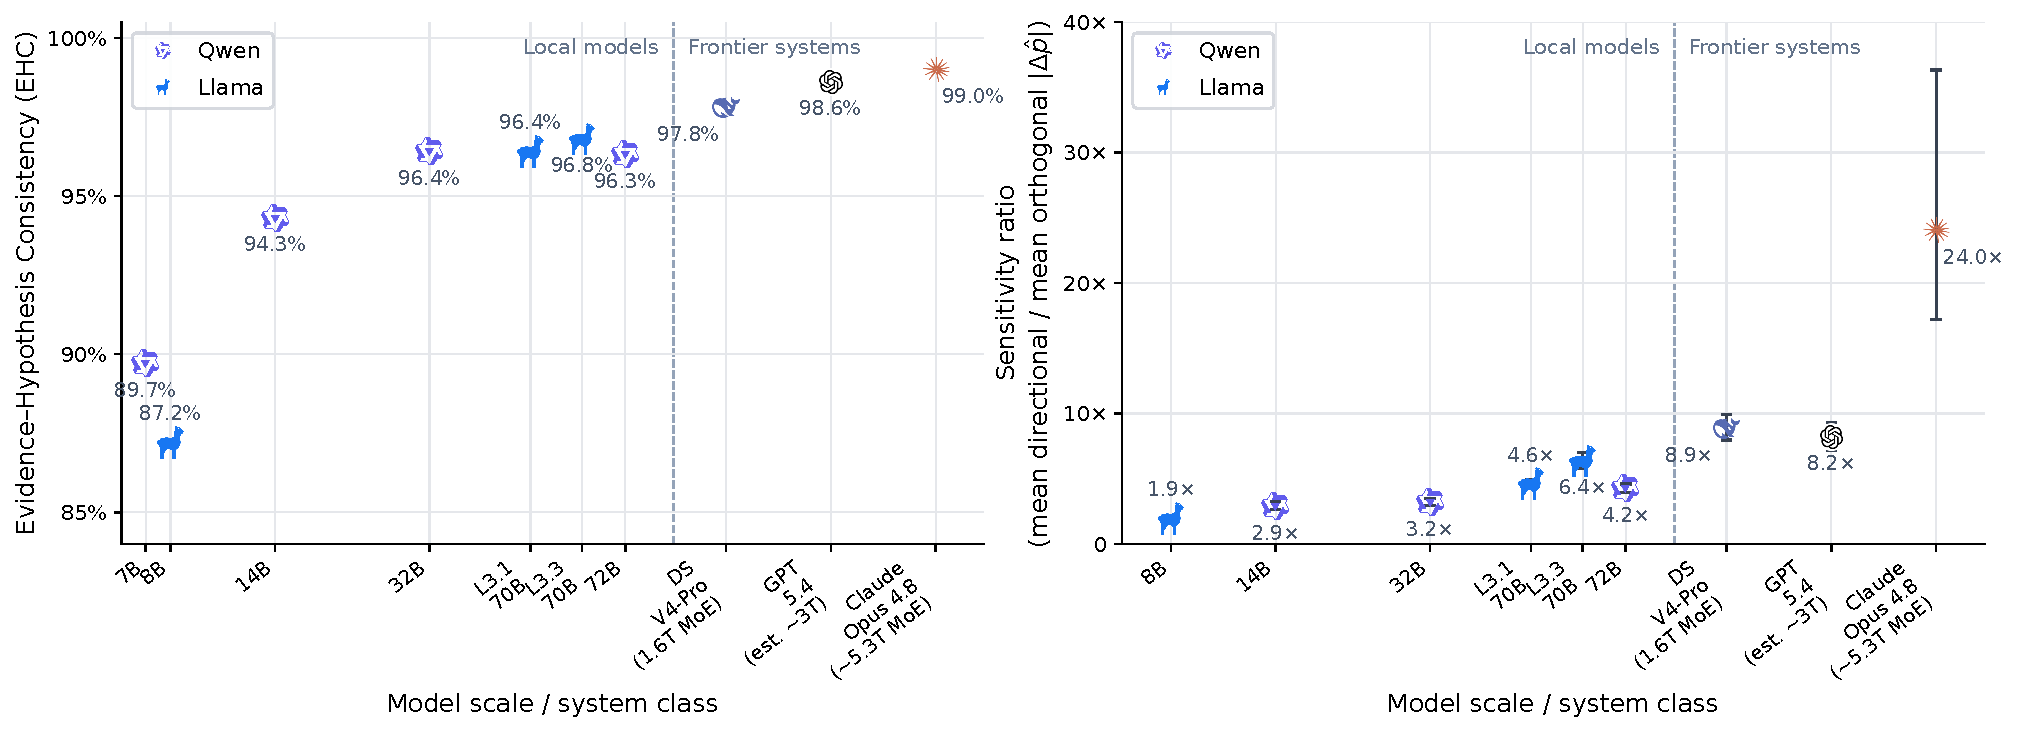
\includegraphics[width=\linewidth]{figures/exp1_ehc_sensitivity_combined.pdf}
\captionof{figure}{\textbf{Directional consistency and packet selectivity by
deployment.} \emph{Left:} EHC is $87$--$90\%$ for 7--8B local models and
$98$--$99\%$ for hosted systems. \emph{Right:} sensitivity is
$1.9$--$6.4\times$ for local models and $8.2$--$24.0\times$ for hosted systems;
Qwen~2.5-7B is omitted from this panel because its archived absolute revisions mix
0--1 and 0--100 scales and therefore do not yield a comparable ratio. The panel
plots the unconditional ratio, which Table~\ref{tab:exp1-abstention} decomposes.}
\label{fig:causal-coherent}
\end{minipage}
\end{center}






\subsection{Study Limitations}
\label{app:exp1-limitations}


\subsubsection{Sampling and Outcome Scope}
The sample is a filtered slice of liquid, medium-horizon Polymarket questions
rather than a probability sample of forecasting tasks. Topic exclusions, the
0.10--0.90 price window, the 14--180 day horizon, event deduplication, and the
diversity cap shape its difficulty distribution.  The primary Experiment~1
estimand evaluates conditional updating on questions that were unresolved at
collection.  The settlement audit in
Section~\ref{app:exp1-outcome-followup} is naturally censored to the first 60
strict settlements and is descriptive.  Experiment~4 separately evaluates
accuracy on a locked sample of resolved historical markets with synchronized
forecast cutoffs and market-price baselines.

\subsubsection{What the Update Prompt Withholds}
\label{app:exp1-withholding}
The Stage~3 template fills in one packet field, \texttt{evidence\_text}. The packet
record also holds the intended \texttt{direction}, \texttt{target\_hypothesis},
\texttt{expected\_hypothesis\_shift}, \texttt{slot\_type}, \texttt{evidence\_headline},
\texttt{mechanism\_targeted}, and a free-text \texttt{rationale}. None of these
reaches the agent; all are read only when the update is scored. The agent sees its
own prior forecast, the snippet, and the fixed instruction.

We checked this two ways. Over the 12{,}728 frozen records that kept their prompt
string, spanning all three hosted systems, the evidence block is identical to the
packet's \texttt{evidence\_text} and contains no private packet field. Prompt
persistence was a per-runner logging choice, so this covers a subset of records by
logging coverage rather than by outcome; the runners that stored nothing use the
same one-field template. Turning to the snippets, none of the 900 names $H_1$,
$H_2$, the market, or its resolution. Twenty-two (2.4\%, 10 pro-$H_1$ and 12
anti-$H_1$) use any likelihood wording---\emph{odds}, \emph{chance of},
\emph{more}/\emph{less likely}, \emph{probability}, \emph{likelihood}---and each
time it describes something in the world, a simulation percentage or a betting
line, not the market's resolution. The sign is not stated; it must be inferred from the relation between the
reported event and the market outcome. Reproduced by
\path{exp1_prospective/agent/audit_packet_polarity.py}.

\subsubsection{Alternative Explanations for the Selectivity Gap}
\label{app:exp1-alternatives}
Here we state the competing accounts of the movement gap and what we find for each.
All checks come from \path{exp1_prospective/agent/audit_selectivity_robustness.py},
\path{audit_orthogonal_abstention.py}, \path{audit_lexical_sign_baseline.py}, and
\path{audit_group_contrast.py}.

\textbf{Where the numbers come from.} The checks read the frozen June~17 report,
which enumerates every scored run, so they use exactly the data behind the
published numbers. The enumeration matches the report's own per-arm counts for
seven of the nine models; Claude Opus~4.8 and GPT-5.4 carry 14 and 4 extra runs in
markets absent from the per-market join, 18 of 38{,}730. Reproduced sensitivity
ratios agree with the published ones to within $0.2$. Three checks need packet
text and so join runs to the June~10 packet set; 346 runs (1.1\%) do not join
because they come from a June~7--8 pilot against a superseded 63-packet
generation, and they are dropped from those three checks only.

\textbf{Attrition is much higher for the hosted systems.} Claude Opus~4.8 made
9{,}313 calls and yielded 3{,}232 usable updates, losing 3{,}656 to broken pipes,
914 to HTTP~401s after a key expired mid-run, and 1{,}481 to unparseable
responses. Of those, 1{,}461 come from one malfunctioning June~15 retry pass that
failed at 91\%; the main June~10 collection parsed at 99.3\%, so the published
compliance figures are not survivorship. DeepSeek~V4-Pro made 6{,}338 calls for
4{,}598 usable updates, losing 1{,}629 to HTTP~401s; GPT-5.4 made 4{,}269 for
4{,}057. The six local models lose almost nothing---four record no failed calls,
the other two lose 8 and 15 responses to parsing. Content-based exclusion is
confined to 28 GPT-5.4 calls across 2 markets. Recorded failures are predominantly
transport or parsing failures; the coverage check below assesses arm and market
imbalance, not content-specific selection. Separately, two
update streams were corrupted by concurrent writes and repaired in August~2026,
after the freeze; the original bytes and unrecoverable fragments sit in
\path{exp1_prospective/data/_recovery_audit/}. Nothing in this section reads those
files.

\textbf{The generator saw one agent's world model.} All packets were built from a
single canonical initial forecast, and it is DeepSeek~V4-Pro's: its June~10 YES
probability matches the stored generation prior on 100 of 100 markets, where no
other agent matches on more than 28. For the other eight models the evidence came
from a different system's event model. The seed model gains nothing by it---among
hosted systems it is second on sensitivity ($8.9\times$ against Claude's
$24.0\times$), third on AUC ($.967$), and last on EHC ($.977$)---but its estimates
are the least independent in the roster.

\textbf{Coverage is uneven across arms.} Table~\ref{tab:exp1-arm-coverage} gives
per-arm market coverage. Seven models cover 99 or 100 markets on every arm. Claude
Opus~4.8 covers 82 on the orthogonal arm and 77 on the directional arms, 73 in
common, so its pooled ratio divides means taken over slightly different market
sets. Restricting to its 73 common markets gives $23.7\times$ against $24.2\times$
pooled. As a proxy check, every other model has similar sensitivity on the markets
Claude covers and those it misses ($8.4$ vs.\
$7.6$ for GPT-5.4, $9.7$ vs.\ $7.2$ for DeepSeek~V4-Pro, $4.3$ vs.\ $4.2$ for
Qwen~2.5-72B, $1.9$ vs.\ $2.1$ for Llama~3.1-8B).

\textbf{The ratio has an unstable denominator.} Claude's orthogonal mean is
$0.5$~pp, so its $24\times$ comes from a small divisor rather than unusually large
directional movement, and its market-clustered interval is correspondingly wide,
$[17.3,36.9]$. Table~\ref{tab:exp1-selectivity-robustness} reports three
statistics that avoid that division. The difference of means is $5.6$--$12.3$~pp
and does not order the models the way the ratio does. The within-market
probability that a directional packet moves the forecast more than an orthogonal
one runs from $.791$ for Llama~3.1-8B to $.994$ for GPT-5.4, putting GPT-5.4 above
Claude Opus~4.8 and reversing the ratio ranking. Every model moves further on
directional packets in every market it covers.

\textbf{The denominator is mostly zeros.} That instability has a specific cause,
and naming it replaces the ratio with two statistics that are easier to read. A
revision of exactly zero---the model reproduces the probability shown to it---enters
the mean like any other record, so the ratio silently mixes how often a
deployment declines to move with how far it moves when it does. Writing $A$ for
the share of runs with $\Delta\hat p=0$ and $M$ for the mean absolute revision
among the rest, $\overline{|\Delta\hat p|}=(1-A)M$, and the ratio factors exactly:
\begin{equation}
  \mathrm{Sensitivity}
  =\underbrace{\frac{M_{\mathrm{dir}}}{M_{\mathrm{orth}}}}_{\text{magnitude}}
  \times\underbrace{\frac{1-A_{\mathrm{dir}}}{1-A_{\mathrm{orth}}}}_{\text{abstention}}.
  \label{eq:sensitivity-decomposition}
\end{equation}
Table~\ref{tab:exp1-abstention} gives both factors. Directional abstention is
$0.0$--$1.4\%$ for every deployment, so the second factor is governed entirely by
the orthogonal arm, where abstention runs from $1.1\%$ for Llama~3.1-8B to
$71.4\%$ $[63.8,78.5]$ for Claude Opus~4.8. Claude's $24\times$ is therefore
$7.0\times$ $[5.5,9.1]$ in magnitude multiplied by $3.48$ in abstention;
DeepSeek~V4-Pro's $8.9\times$ is $4.9\times$ times $1.79$; GPT-5.4's $8.2\times$
is $7.5\times$ times $1.09$, because GPT-5.4 writes a small revision where the
other two hosted systems return the prior unchanged. Across the roster the
published $1.9$--$24.2\times$ becomes $1.9$--$7.5\times$ once the zeros are
separated out, and the ordering changes: GPT-5.4 rather than Claude Opus~4.8 is
highest, and Llama~3.3-70B at $5.7\times$ sits above DeepSeek~V4-Pro at
$4.9\times$.

We report both factors rather than the product. Declining to revise at all is an
appropriate response to an outcome-irrelevant premise, so the abstention rate is
a selectivity measure in its own right and a better-behaved one: it is a bounded
proportion, it is paired within model across arms, and it needs no division by a
small number. It is also the more fragile of the two. An exact copy of a
displayed prior is a discrete act adjacent to formatting, and the update prompt
does instruct the agent to leave unaffected fields unchanged, so we do not read a
high rate as evidence about internal computation. The no-information condition
described in Section~\ref{app:exp1-limitations} is what would separate declining
to revise from copying the anchor, and it was not run. Reproduced by
\path{exp1_prospective/agent/audit_orthogonal_abstention.py}.

\begin{center}
\begin{minipage}{\linewidth}
\centering
\captionof{table}{Decomposition of the sensitivity ratio into magnitude and
abstention factors (Equation~\ref{eq:sensitivity-decomposition}). \emph{Orthogonal
abstention} is the share of orthogonal runs with $\Delta\hat p$ exactly zero; the
directional-arm rate is $0.0$--$1.4\%$ throughout. The two \emph{given a move}
columns condition on a nonzero revision, and their ratio is the magnitude factor.
Brackets are 95\% market-clustered percentile intervals from 20,000 draws, the
scheme used for the published movement intervals. Qwen~2.5-7B is omitted for
mixed probability scales.}
\label{tab:exp1-abstention}
\scriptsize
\setlength{\tabcolsep}{4pt}
\resizebox{\linewidth}{!}{%
% Generated by exp1_prospective/agent/audit_orthogonal_abstention.py; do not edit.
\begin{tabular}{lccccc}
\toprule
& \textbf{Orthogonal} & \multicolumn{2}{c}{\textbf{Mean $|\Delta\hat p|$ given a move}} & \textbf{Sens.} & \textbf{Sens.} \\
\cmidrule(lr){3-4}
\textbf{Model} & \textbf{abstention} & orthogonal & directional & \textbf{given a move} & \textbf{published} \\
\midrule
Claude Opus~4.8  & 71.4\% {\scriptsize[63.8,\,78.5]} & 1.6\,pp & 11.2\,pp & $7.0\times$ {\scriptsize[5.5,\,9.1]} & $24.2\times$ {\scriptsize[17.3,\,36.9]} \\
GPT-5.4          & 8.4\% {\scriptsize[5.2,\,11.9]} & 1.3\,pp & 9.6\,pp & $7.5\times$ {\scriptsize[6.6,\,8.5]} & $8.2\times$ {\scriptsize[7.2,\,9.3]} \\
DeepSeek V4-Pro  & 44.4\% {\scriptsize[38.9,\,50.0]} & 2.6\,pp & 12.7\,pp & $4.9\times$ {\scriptsize[4.4,\,5.5]} & $8.9\times$ {\scriptsize[8.0,\,9.9]} \\
\midrule
Qwen~2.5-72B     & 24.2\% {\scriptsize[19.6,\,29.0]} & 3.9\,pp & 12.6\,pp & $3.2\times$ {\scriptsize[3.0,\,3.4]} & $4.2\times$ {\scriptsize[3.9,\,4.6]} \\
Llama~3.3-70B    & 10.7\% {\scriptsize[7.0,\,14.8]} & 2.6\,pp & 14.6\,pp & $5.7\times$ {\scriptsize[5.2,\,6.2]} & $6.4\times$ {\scriptsize[5.8,\,7.0]} \\
Llama~3.1-70B    & 2.5\% {\scriptsize[0.8,\,5.0]} & 3.4\,pp & 15.2\,pp & $4.5\times$ {\scriptsize[4.2,\,4.8]} & $4.6\times$ {\scriptsize[4.3,\,4.9]} \\
Qwen~2.5-32B     & 11.1\% {\scriptsize[8.0,\,14.6]} & 4.5\,pp & 12.6\,pp & $2.8\times$ {\scriptsize[2.6,\,3.1]} & $3.2\times$ {\scriptsize[2.9,\,3.5]} \\
Qwen~2.5-14B     & 26.1\% {\scriptsize[20.7,\,31.9]} & 5.5\,pp & 11.9\,pp & $2.2\times$ {\scriptsize[2.0,\,2.3]} & $2.9\times$ {\scriptsize[2.6,\,3.2]} \\
Llama~3.1-8B     & 1.1\% {\scriptsize[0.5,\,1.9]} & 6.0\,pp & 11.6\,pp & $1.9\times$ {\scriptsize[1.8,\,2.0]} & $1.9\times$ {\scriptsize[1.8,\,2.1]} \\
\bottomrule
\end{tabular}

}
\end{minipage}
\end{center}

\textbf{The deployment contrast depends on the statistic.} Comparing the three
hosted systems against the six scale-valid open-weight models by market-clustered
bootstrap (20{,}000 replicates, macro-averaged within group so a model with more
runs does not dominate), the statistics disagree. On the ratio the
difference is $+9.8$ $[7.2,14.2]$, group means $13.7\times$ and $3.9\times$, and
the per-model ranges do not overlap. On AUC it is $+.070$ $[.062,.079]$, which
excludes zero, but the ranges do overlap: Llama~3.3-70B at $.989$ and
Llama~3.1-70B at $.978$ both beat DeepSeek~V4-Pro at $.967$. On raw movement there
is no difference at all, $+0.8$ $[-0.0,1.7]$~pp around means of $10.1$ and $9.3$.

The decomposition explains why the ratio is the one statistic that separates the
groups completely. Both of its factors favour the hosted systems on average and
neither separates them on its own: orthogonal abstention differs by $+.286$
$[.244,.329]$ around group means of $.413$ and $.126$, with four open-weight
deployments at or above GPT-5.4's $8.4\%$; the magnitude factor differs by
$+3.10$ $[2.31,4.08]$ around $6.5\times$ and $3.4\times$, with Llama~3.3-70B
above DeepSeek~V4-Pro. Multiplying two partially separating factors yields a
product whose ranges happen not to overlap, so we do not report that non-overlap
as a finding. The two classes move about equally far on directional evidence; the
hosted systems more often decline to move at all on controls, and move somewhat
less far when they do. We state the deployment result that way rather than as a
general selectivity ordering. Group contrasts come from
\path{exp1_prospective/agent/audit_group_contrast.py}.

\textbf{The arms differ in wording.} By construction directional packets take the
DATA, DECISION, and STRUCTURAL slots and orthogonal packets take PROCEDURAL,
PERSONNEL, and BACKDROP, and the text differs accordingly: directional snippets
average $96.8$ words and $7.1$ digits, orthogonal ones $85.7$ and $3.7$. Movement
could track density rather than content. Two checks argue otherwise. Within the
directional arm, where length cannot indicate sign, Spearman correlation between
word count and $|\Delta\hat p|$ is $-.06$ to $.00$ and between digit count and
$|\Delta\hat p|$ is $.01$ to $.10$. And the arms' word counts almost fully overlap
(orthogonal 66--114, directional 66--121); restricting to that band keeps 889 of
900 packets and moves every sensitivity estimate by at most $0.1$
(Table~\ref{tab:exp1-selectivity-robustness}, last column). The arms are not
matched on surface form. These checks show that word and digit counts do not
explain the effect; other surface differences remain. Directional correctness is
not explained by length, since length cannot say which way to move.

\textbf{A shallow classifier might be enough.} We tested it. Multinomial naive
Bayes and L2-regularised logistic regression were fit on the 900 packet texts with
five-fold cross-validation grouped by market, so no market appears on both sides
of a fold. Telling directional from orthogonal packets is nearly free: naive Bayes
reaches $.989$ against a $.667$ majority rate. That follows from the slot-type
plan rather than revealing anything---the most distinctive orthogonal tokens are
\emph{appointed}, \emph{appointment}, \emph{oversee}, and \emph{accreditation},
which name the roles the generator was told to write. So a model could route on
that marking without weighing content, and the sensitivity ratio alone cannot rule
it out. Matching the control arm on evidence type would need a different packet
design; the checks above bound only the length part of the problem.

Recovering the \emph{sign} is another matter. On pro-$H_1$ versus anti-$H_1$ the
same classifiers reach $.688$ and $.675$ against $.500$ chance, and prepending the
market question does not help ($.665$ and $.680$): these bag-of-words models do
not combine question polarity with event valence. The tokens it keys on carry no
consistent sign---\emph{vessel}, \emph{venue}, \emph{signature} for pro-$H_1$,
\emph{table}, \emph{materials}, \emph{findings} for anti-$H_1$. Against this $.69$ lexical baseline, the human panel reaches $.762$ on its
smaller categorical task and the hosted agents $.973$--$.984$ on probability
revision. These are not matched performance comparisons. The agent--classifier gap
is evidence against this bag-of-words account, not proof that no surface heuristic
can recover sign; unlike the arm contrast, it stays within pro- versus anti-$H_1$
packets.

\textbf{Does the stated reasoning track the packet?} If movement were routed on
surface marking, a model's written rationale would not need to bear any particular
relation to what it does with the forecast. We tested two versions of this
(\path{exp1_prospective/agent/audit_mechanism_tracking.py}).

The first asks whether a rationale identifies the specific mechanism its packet was
built to target, ranking the true \texttt{mechanism\_targeted} against the other
eight from the same market so that question, actors, and domain vocabulary are held
fixed. Rationales rank it first on $.278$--$.430$ of records against $1/9$ chance,
but the snippet alone scores $.516$, so most of that is echo of the text the model
just read. Removing every token the snippet supplied leaves $.128$--$.195$ under
matched query length, still above chance---but the generator's own rationale for
the packet, scored the same way, lands at $.119$, essentially chance, because it
paraphrases the mechanism rather than restating it. With the reference writer at
chance the metric has no usable dynamic range, and we draw no conclusion from it.

Models often declare orthogonal packets irrelevant: explicit non-relevance wording appears in
$4.9$--$61.9\%$ of orthogonal rationales against $0.1$--$2.8\%$ of directional
ones. What matters is whether saying it predicts doing it. Within the orthogonal
arm, records whose rationale declares irrelevance move less than those that do not,
and the market-clustered gap excludes zero for eight of the nine scale-valid
deployments: $0.88$~pp $[0.56,1.22]$ for Claude Opus~4.8, $1.70$
$[1.45,1.96]$ for DeepSeek~V4-Pro, $2.73$ $[2.28,3.19]$ for Qwen~2.5-72B, down to
$0.36$ $[0.21,0.54]$ for GPT-5.4, whose unflagged orthogonal movement is already
$1.3$~pp. The exception is Llama~3.1-8B at $0.26$ $[-0.64,1.06]$, where no coupling is
detectable; it is also the weakest deployment on sensitivity and directional
correctness, though we do not test whether the two are related. Qwen~2.5-7B is
omitted for mixed probability scales.

For eight of nine deployments, then, the revision a model makes is not independent
of the relevance it states, and the one deployment where that link is undetectable
is the weakest on every other measure. Two limits: the flag is a hand-built
lexicon, so it captures what a rationale declares rather than what the model
understood; and consistent self-description is compatible with surface routing, so
this does not show relevance was derived from the mechanism.

\textbf{One deployment was prompted differently.} GPT-5.4, and only GPT-5.4,
received the \texttt{novelty\_assessment} rule at Stage~3
(Section~\ref{app:update-protocol}).  Because that rule speaks directly to revision
size, its abstention rate is not comparable to the other deployments'. The
within-GPT contrast uses one template, but the extra instruction could interact
with packet arm, so its contrast should not be attributed to model differences
alone.

\textbf{Two remaining caveats.} A single generator wrote all packets and scored its
own work at a uniform 4/5 for plausibility, so automated validation establishes
structural completeness but not equal difficulty or independent content validity.
And the local models ran through Ollama at the default tag for each name, with the
served weight precision not recorded per run; rows ordered by parameter count also
vary in quantization and inference stack, so we do not attribute the open-weight
ordering to parameter count alone.

\begin{center}
\begin{minipage}{\linewidth}
\centering
\captionof{table}{Per-arm market coverage in the frozen June~17 report. Markets
counts entries in the model's per-market block, which for three Qwen rows
includes 20 carrying no scored update; the arm columns count markets with at
least one.}
\label{tab:exp1-arm-coverage}
\small
\begin{tabular}{lcccc}
\toprule
\textbf{Model} & \textbf{Markets} & \textbf{pro-$H_1$/anti-$H_1$} & \textbf{orthogonal} & \textbf{all three} \\
\midrule
Claude Opus~4.8 & 100 & 77 & 82 & 73 \\
GPT-5.4         & 100 & 99 & 99 & 99 \\
DeepSeek V4-Pro & 100 & 100 & 100 & 100 \\
\midrule
Qwen~2.5-72B    & 120 & 100 & 100 & 100 \\
Llama~3.3-70B   & 100 & 100 & 100 & 100 \\
Llama~3.1-70B   & 100 & 99 & 99 & 99 \\
Qwen~2.5-32B    & 120 & 100 & 100 & 100 \\
Qwen~2.5-14B    & 120 & 100 & 100 & 100 \\
Llama~3.1-8B    & 100 & 100 & 100 & 100 \\
\bottomrule
\end{tabular}
\end{minipage}
\end{center}

\begin{center}
\begin{minipage}{\linewidth}
\centering
\captionof{table}{Selectivity under statistics that do not divide by the orthogonal
mean. \emph{Sens.} is the frozen ratio; \emph{Diff.} is mean directional minus mean
orthogonal absolute revision; \emph{AUC} is the within-market probability that a
directional packet moves the forecast more than an orthogonal one, averaged over
markets; \emph{Markets} counts markets where mean directional movement exceeds
mean orthogonal movement; \emph{Length-m.} recomputes the ratio on the 66--114-word
band the arms share. Qwen~2.5-7B is omitted for mixed probability scales.}
\label{tab:exp1-selectivity-robustness}
\small
\begin{tabular}{lccccc}
\toprule
\textbf{Model} & \textbf{Sens.} & \textbf{Diff.} & \textbf{AUC} & \textbf{Markets} & \textbf{Length-m.} \\
\midrule
Claude Opus~4.8  & $24.0\times$ & 10.7\,pp & 0.984 & 77/77 & $24.3\times$ \\
GPT-5.4          & $8.2\times$ & 8.4\,pp & 0.994 & 99/99 & $8.1\times$ \\
DeepSeek V4-Pro  & $8.9\times$ & 11.2\,pp & 0.967 & 100/100 & $8.8\times$ \\
\midrule
Qwen~2.5-72B     & $4.2\times$ & 9.6\,pp & 0.950 & 100/100 & $4.2\times$ \\
Llama~3.3-70B    & $6.4\times$ & 12.3\,pp & 0.989 & 100/100 & $6.4\times$ \\
Llama~3.1-70B    & $4.6\times$ & 11.9\,pp & 0.978 & 99/99 & $4.6\times$ \\
Qwen~2.5-32B     & $3.2\times$ & 8.7\,pp & 0.906 & 100/100 & $3.2\times$ \\
Qwen~2.5-14B     & $2.9\times$ & 7.7\,pp & 0.852 & 100/100 & $2.9\times$ \\
Llama~3.1-8B     & $1.9\times$ & 5.6\,pp & 0.791 & 100/100 & $1.9\times$ \\
\bottomrule
\end{tabular}

\end{minipage}
\end{center}

\subsubsection{Human Materials Review}
\label{app:exp1-human-review}
Nine adult reviewers submitted the 18-item materials protocol. It samples one
report from each of 18 distinct markets, balanced across six pro-YES, six
anti-YES, and six orthogonal packets. One reviewer met the disclosed
response-pattern exclusion below, leaving eight quality-eligible reviewers.
We treat the study as descriptive materials evidence. Before the synthetic
report, every item shows the market question,
resolution criteria, and matching summary from the frozen June~10 initial
forecast. The consent screen and every item instruct reviewers to treat
June~10, 2026 as the current date and use no external information or assistance.
Intended directions, source IDs, generator
metadata, and model responses remain hidden.

Reviewers record the report's conditional direction, confidence, clarity,
real-world plausibility, and usability as an explicit hypothetical premise.
We report exact agreement with the frozen direction and Cohen's $\kappa$
between the panel-majority labels and the frozen key. Reviewer-level Cohen's
$\kappa$, the component ratings, and every item-level judgment appear below.
Ambiguous judgments remain in every denominator.

Practice responses are stored separately and excluded from the analysis.

The analyzed sample contains eight quality-eligible reviewers (R1 and R3--R9),
exceeding the six-reviewer target for this descriptive materials check.
Table~\ref{tab:stage3-human} includes every eligible reviewer.

Exact-direction agreement is 108/144 (75.0\%). The panel-majority label matches
the frozen direction on 17 of 18 items (94.4\%; Cohen's $\kappa=.919$): all six
anti-$H_1$ items, all six orthogonal items, and five of six pro-$H_1$ items.
Across individual judgments, exact agreement is 35/48 for pro-$H_1$, 37/48 for
anti-$H_1$, and 36/48 for orthogonal packets. Reviewers marked the premise usable
on 124/144 judgments (86.1\%). The corresponding all-reviewer sensitivity is
reported below. These descriptive results indicate that readers usually recovered
the intended conditional direction and could use the reports as stipulated premises.
They also bound how legible that direction is: 75.0\% exact agreement and mean
pairwise Cohen's $\kappa=.47$ indicate substantial but imperfect recovery across
the four response labels. The panel is not a matched baseline for the agents---reviewers
emit a categorical label on 18 items, agents emit a revised probability against
their own prior on all 900---so we read it as evidence that sign had to be
inferred, not as a human--model comparison.
\begin{center}
\begin{minipage}{\linewidth}
\centering
\small
\captionof{table}{\textbf{Stage~3 human materials judgments for eight quality-eligible reviewers.}
Direction is exact agreement with the frozen conditional direction and
$\kappa$ is Cohen's $\kappa$ against that key over the four response options.
Confidence, clarity, and plausibility (C/C/P) are reviewer-level medians on 1--5
scales. The pooled row is descriptive because reviewers rated the same items; the
majority row takes the modal label per item, resolving ties to \emph{ambiguous}.}
\label{tab:stage3-human}
\begin{tabular}{lcccc}
\toprule
Reviewer & Direction agreement & $\kappa$ vs. key & Premise usable & C/C/P \\
\midrule
R1 & 12/18 (66.7\%) & .54 & 10/18 & 4/4/4 \\
R3 & 12/18 (66.7\%) & .51 & 13/18 & 4/4/3 \\
R4 & 18/18 (100.0\%) & 1.00 & 18/18 & 5/5/5 \\
R5 & 10/18 (55.6\%) & .38 & 18/18 & 4/4/4 \\
R6 & 13/18 (72.2\%) & .61 & 12/18 & 4/4/5 \\
R7 & 15/18 (83.3\%) & .76 & 17/18 & 5/4/3 \\
R8 & 12/18 (66.7\%) & .55 & 18/18 & 4/5/4 \\
R9 & 16/18 (88.9\%) & .84 & 18/18 & 5/5/5 \\
\midrule
Pooled & 108/144 (75.0\%) & --- & 124/144 & --- \\
Majority label & 17/18 (94.4\%) & .92 & --- & --- \\
\bottomrule
\end{tabular}
\end{minipage}
\end{center}

\begin{center}
\begin{minipage}{\linewidth}
\centering
\scriptsize
\setlength{\tabcolsep}{3pt}
\captionof{table}{\textbf{Item-level Stage~3 judgments for eight quality-eligible reviewers.}
Key is the frozen conditional direction; Majority is the modal panel response,
with ties assigned to \emph{ambiguous}. Agree and Usable give counts out of eight;
C/L/P gives median direction confidence, clarity, and plausibility on 1--5 scales.
Item numbers follow the frozen public packet order.}
\label{tab:stage3-items}
\begin{tabular}{@{}p{.40\linewidth}llccc@{}}
\toprule
Question & Key & Majority & Agree & C/L/P & Usable \\
\midrule
1. Hormuz traffic normal by July 31 & More & More & 8/8 & 5/5/4.5 & 8/8 \\
2. Iran reaches World Cup knockouts & Less & Less & 6/8 & 4.5/4.5/4.5 & 7/8 \\
3. Israel strikes Yemen by June 30 & No effect & No effect & 8/8 & 4.5/4/3.5 & 6/8 \\
4. Netanyahu exits election by July 31 & More & More & 6/8 & 5/5/4.5 & 8/8 \\
5. Anthropic valuation reaches \$1.1T & Less & Less & 7/8 & 4.5/4.5/5 & 8/8 \\
6. Oladokun starts Chiefs Week 1 & No effect & No effect & 6/8 & 4/4/3.5 & 7/8 \\
7. S\&P 500 reaches 7,700 in June & More & More & 4/8 & 3.5/4/5 & 7/8 \\
8. Trump unfreezes Iranian assets & Less & Less & 5/8 & 3.5/4/4 & 7/8 \\
9. May durable-goods orders: 0--2\% & No effect & No effect & 4/8 & 3/3/3.5 & 6/8 \\
10. China Q2 growth: 4.6--4.9\% & More & Ambig. & 3/8 & 3/4/3.5 & 5/8 \\
11. Eisenkot joins Bennett--Lapid alliance & Less & Less & 6/8 & 5/5/5 & 7/8 \\
12. Russia enters Orikhiv by July 31 & No effect & No effect & 8/8 & 5/4/4.5 & 6/8 \\
13. Romanian PM is independent/technocrat & More & More & 6/8 & 4.5/4.5/4 & 8/8 \\
14. Russia captures Kostyantynivka & Less & Less & 5/8 & 3.5/5/5 & 7/8 \\
15. At least four June ChatGPT outages & No effect & No effect & 4/8 & 3/4/4 & 7/8 \\
16. El-Sayed wins Michigan primary & More & More & 8/8 & 5/5/5 & 8/8 \\
17. Little is MN-02 Democratic nominee & Less & Less & 8/8 & 5/5/4 & 7/8 \\
18. OpenAI IPO close: \$1.25--1.5T & No effect & No effect & 6/8 & 4/3.5/3.5 & 5/8 \\
\bottomrule
\end{tabular}

\end{minipage}
\end{center}


The response-pattern quality rule excludes any reviewer who selects one direction
on at least 17 of 18 balanced items. R2 met this rule by selecting \emph{more
likely} on 17 of 18 balanced items, including all six frozen negative items
and five of six frozen null items. Raw responses are retained, and no item is
removed or relabeled. Retaining R2 gives 115/162 (71.0\%) exact agreement across
all nine reviewers.


The task requests no identifying or sensitive information. It was conducted as
an internal materials review under the authors' institutional guidance; no IRB
protocol was opened.

Figure~\ref{fig:exp1-review-interface} records the reviewer-facing workflow. The
capture script at
\path{exp1_prospective/stage3_materials_annotation/capture_review_screenshots.py}
loads the frozen item packet against an empty temporary annotation database.
Item order was independently randomized by reviewer.


\begin{figure}[p]
\centering
\begin{subfigure}[t]{0.36\linewidth}
  \centering
  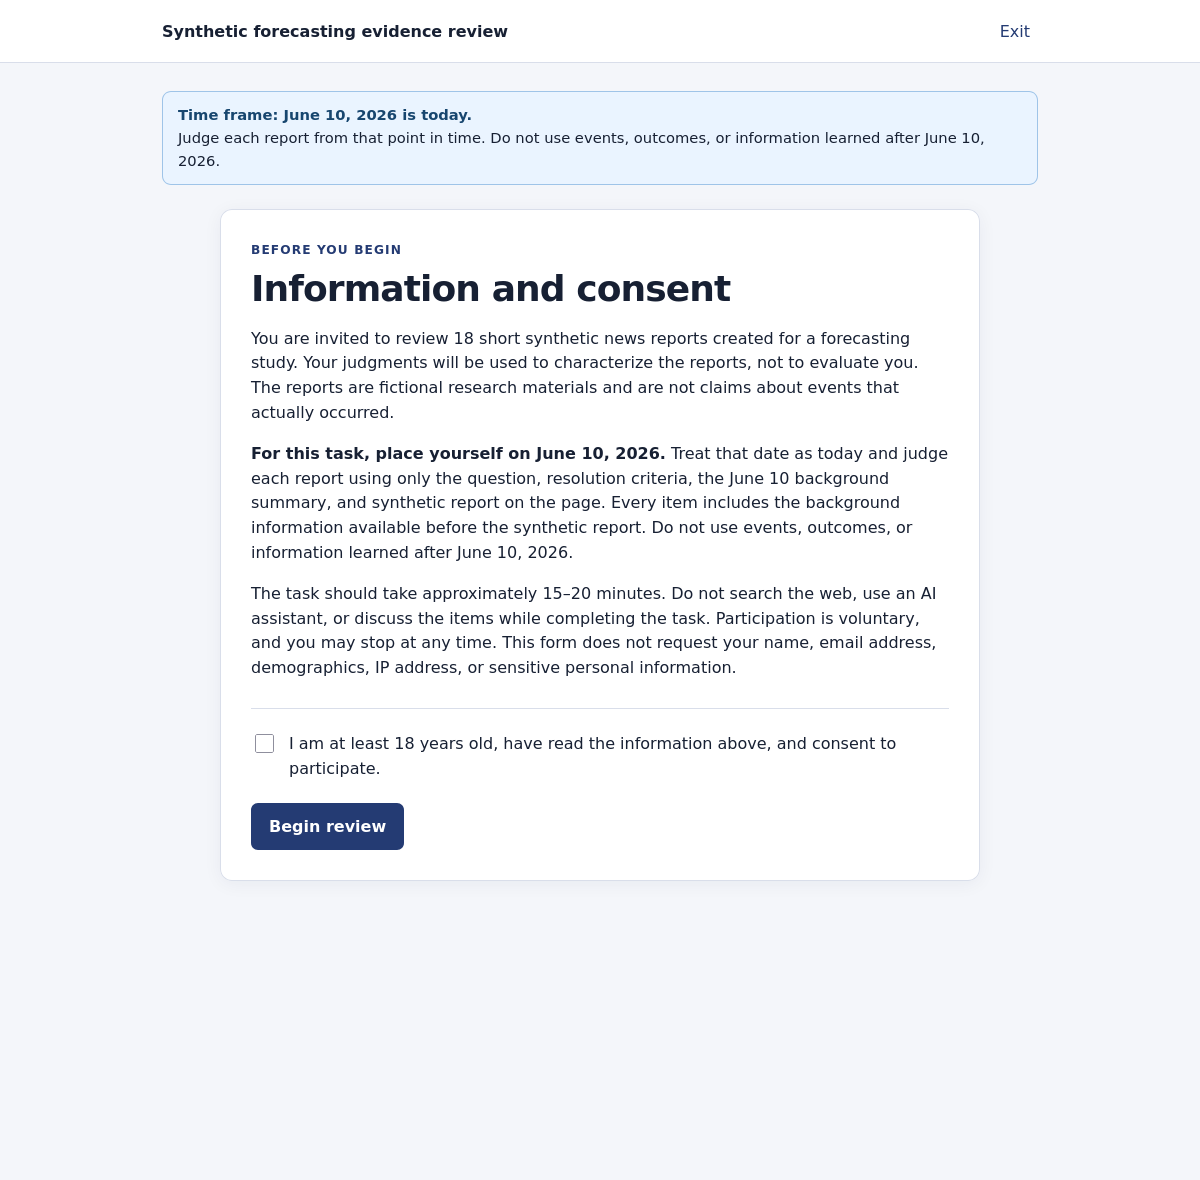
\includegraphics[width=\linewidth]{figures/exp1_stage3_review_consent.png}
  \caption{Information, temporal frame, and consent.}
\end{subfigure}\hfill
\begin{subfigure}[t]{0.60\linewidth}
  \centering
  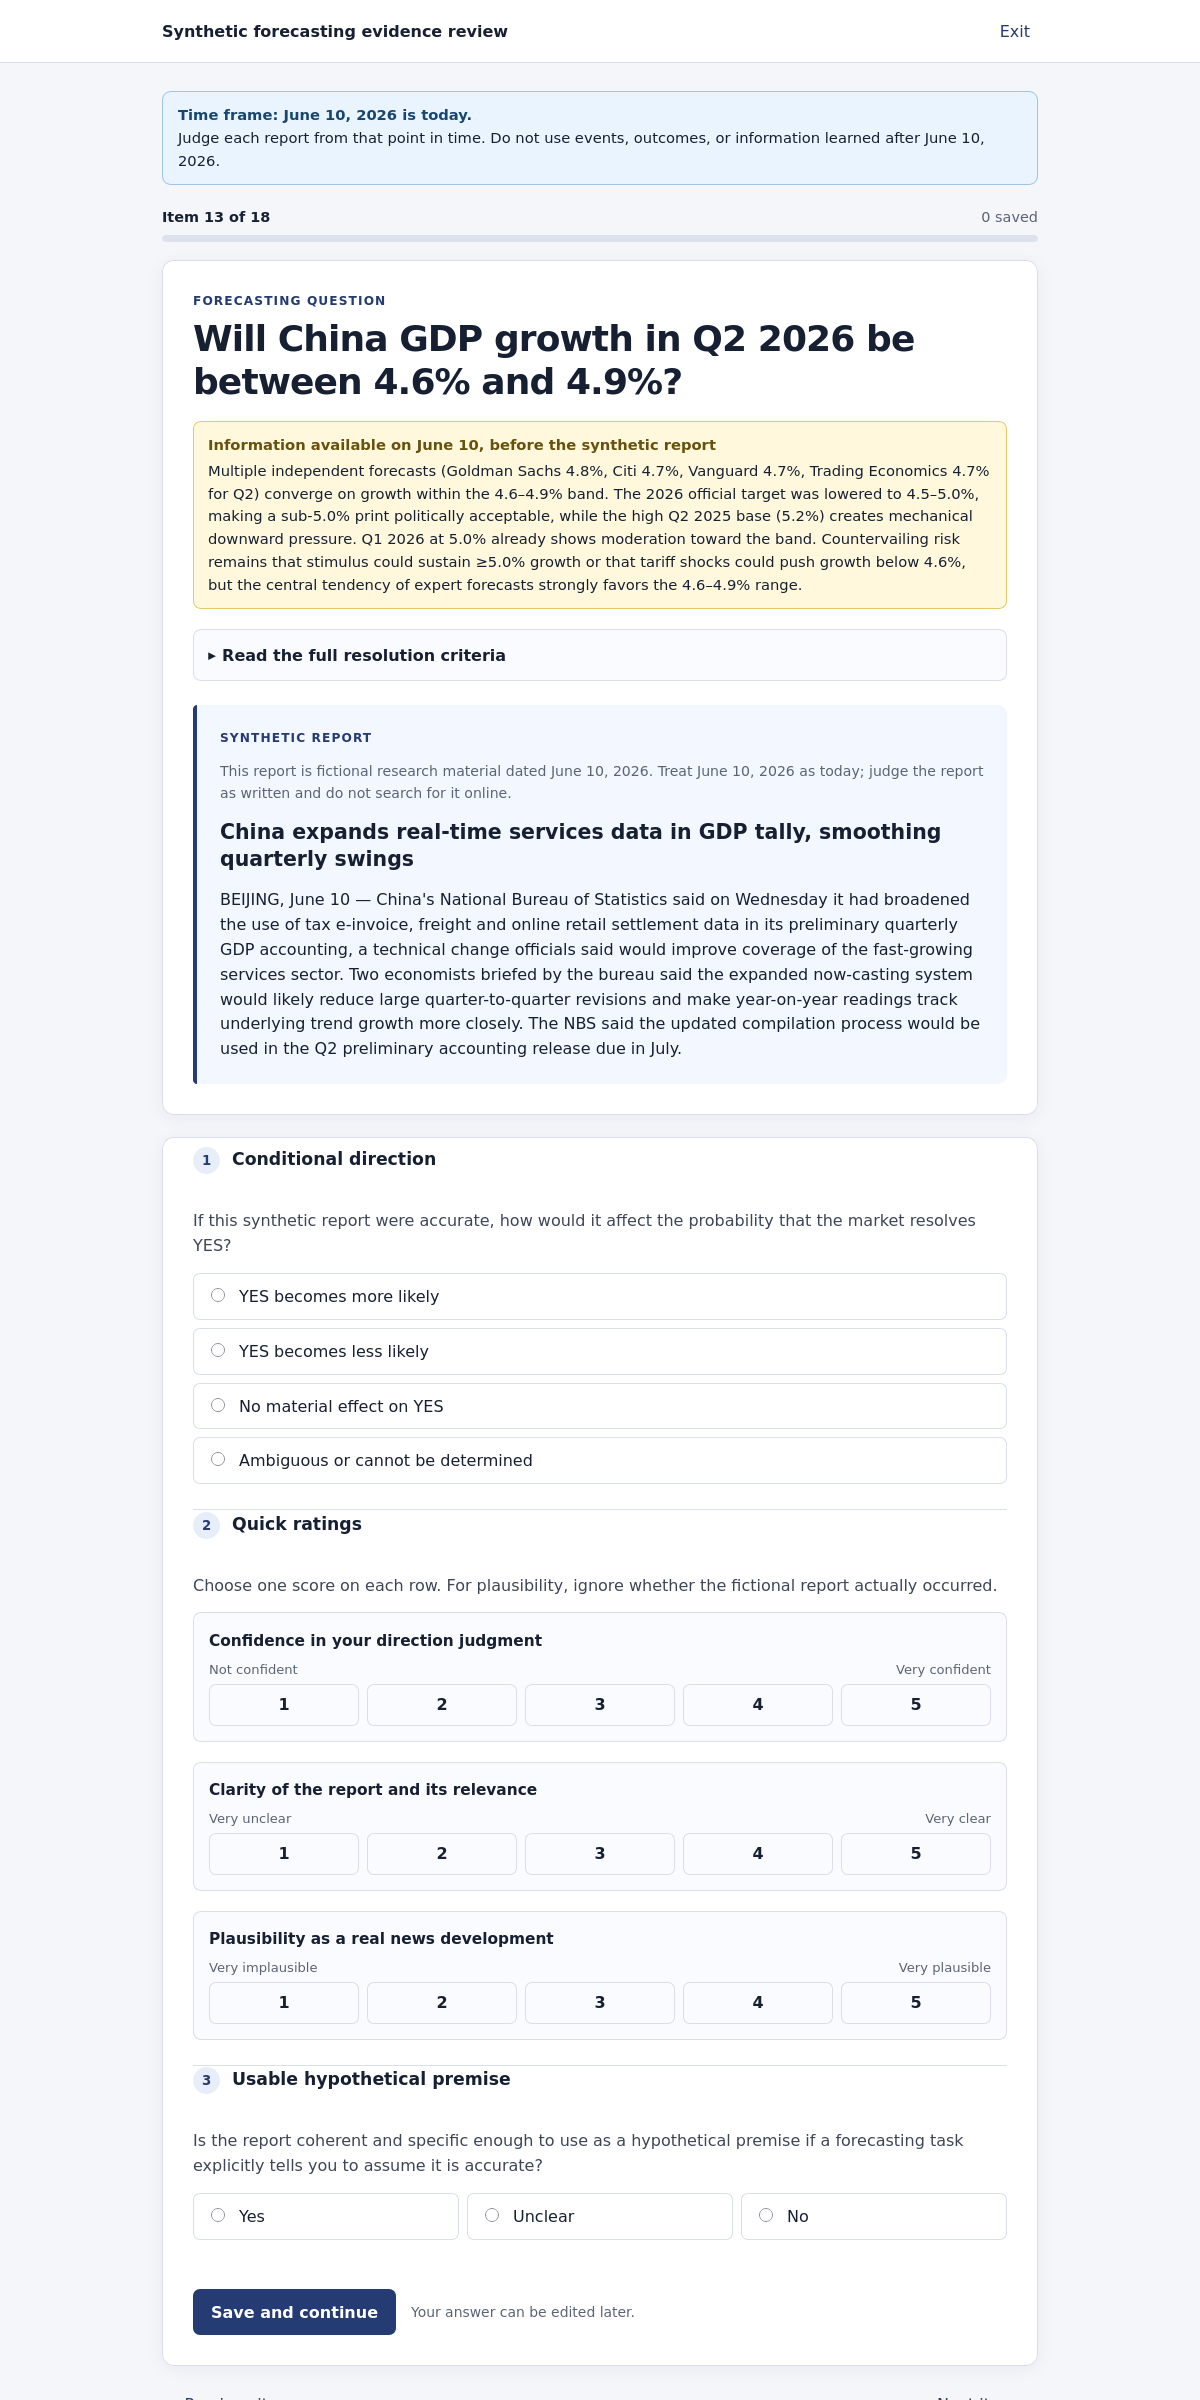
\includegraphics[width=\linewidth]{figures/exp1_stage3_review_item.png}
  \caption{A complete item with June~10 context, synthetic report, and five judgments.}
\end{subfigure}
\caption{\textbf{Stage~3 materials-review interface.} Reviewers enter a private
code before seeing the information-and-consent screen. Each item repeats the
June~10 temporal frame, presents the question and pre-report background, labels
the fictional evidence as a synthetic report, and collects conditional
direction, confidence, clarity, plausibility, and premise usability. Item order
was independently randomized by reviewer. Intended direction and private packet
metadata are hidden.}
\label{fig:exp1-review-interface}
\end{figure}

Orthogonal packets are a useful outcome-relevance control, but are not equivalent
to receiving no new text. A literal no-information update condition would separate
generic prompt-induced revision from response to topically adjacent content.  The very
small hosted-system orthogonal revisions (0.5--1.4~pp) do not substitute for
that control.

\subsubsection{Prompt, Retrieval, and Runtime Confounding}
Agents shared a substantive task contract, while execution was not byte-identical. Hosted
models used Azure Foundry search, while local models used Tavily results in an
Ollama workflow; temperatures and provider behavior also differ. Hosted--local
gaps therefore combine model capability with retrieval and runtime differences.

\subsubsection{Scale, Missingness, and Dependence}
Realized repeat counts are uneven because failures and top-ups differ by provider.
Equal-weight market aggregation prevents high-coverage markets from dominating
EHC, HFC, and ICS. Movement and sensitivity intervals use 20,000
market-clustered bootstrap draws that retain every packet and repeated initial-run
update from each selected market. The mixed-scale Qwen~2.5-7B row described in
Section~\ref{app:record-processing} remains an appendix compliance diagnostic and is
excluded from the main magnitude comparison.

\subsubsection{Premise Acceptance at Stage~3}
Search is intentionally unavailable during updating, and agents are told to
accept the synthetic headline as true. This design measures conditional premise
use rather than source verification or epistemic refusal. The human materials review
uses the same instruction and therefore assesses comprehension and premise
usability. These results do not establish whether a model should trust or verify
the synthetic report.

\subsection{Reproducibility and Artifact Map}
\label{app:fig-code}

The paper treats the June~17 model-update report and the August~23 final
materials-review summary as the frozen numerical authorities. The relevant
artifacts are:

\begin{itemize}
  \item \textbf{Sampling:}
        \path{exp1_prospective/fetch_markets/select_markets.py} and the June~9
        selection/diversity JSON and manifests in
        \path{exp1_prospective/data/selected_markets/}.
  \item \textbf{Initial elicitation:}
        \path{exp1_prospective/agent/forecast_agent.py} for hosted runs and
        \path{exp1_prospective/agent/run_local_forecast.py} for Ollama runs, with
        records and manifests in \path{exp1_prospective/data/initial_forecasts/}.
  \item \textbf{Interventions:}
        \path{exp1_prospective/agent/build_counterfactuals.py} and the frozen
        \path{exp1_prospective/data/counterfactuals/counterfactuals_2026-06-10.jsonl}.
  \item \textbf{Updates:}
        hosted and local update runners under \path{exp1_prospective/agent/}, with
        update records in \path{exp1_prospective/data/updated_forecasts/}.
  \item \textbf{Evaluation:}
        \path{exp1_prospective/agent/evaluate_consistency.py} and
        \path{exp1_prospective/data/results/consistency_report_2026-06-17.json};
        \path{exp1_prospective/agent/evaluate_clustered_uncertainty.py}
        reconstructs the 20,000-draw market-clustered intervals in
        \path{exp1_prospective/data/results/clustered_movement_uncertainty.json};
        \path{exp1_prospective/agent/audit_orthogonal_abstention.py} writes the
        abstention/magnitude decomposition of Table~\ref{tab:exp1-abstention} to
        \path{exp1_prospective/data/results/orthogonal_abstention.json} and its
        table source, under the same resampling scheme.
  \item \textbf{Human materials review:}
        the frozen protocol, blinded packet, browser application, and tests in
        \path{exp1_prospective/stage3_materials_annotation/};
        \path{make_final_summary.py} reconstructs
        \path{data/exports/final_summary_current.json}, while
        \path{data/exports/agreement_current.json} is the paper-facing agreement
        export.
  \item \textbf{Figures:}
        \path{paper/generate_figures.py} writes the direction-selective panel;
        \path{paper/generate_paper_figures.py} writes the combined
        EHC/sensitivity panel.
\end{itemize}

The model-update tables are defined by the June~17 frozen JSON. The mutable collection
directories contain later records, so evaluating their present contents would
define a different dataset. Bit-for-bit reconstruction begins from the frozen
JSON; a full pipeline reconstruction uses only the manifests and records included
in that freeze.
